\scanpage{34}
% archive sheet number: 33
\[
\begin{aligned}
F_3&=T\\
F_4&=T-1\\
F_5&=T^2-T-1\\
F_6&=T-2
\end{aligned}
\]
On peut définir $F_n$ comme le polynôme minimal (sur $\mathbb Q$) de $1+2\cos 2\pi/n$, \deleted{\unsure{de $1+$}} ou encore de $1+\zeta+\zeta^{-1}$, où $\zeta$ est une racine \uline{primitive} $n$.ième de l'unité.

\noindent\rule{.88\linewidth}{.3pt}
\diagram{\begin{tikzcd}[ampersand replacement=\&,column sep=small]
\zeta_0\arrow[r,"\underbrace{\hspace{1.4em}}_{e_1}"']\& \zeta_1\&\zeta_2\&\zeta_3
\end{tikzcd}}
\[
\begin{aligned}
\zeta_1-\zeta_0&=e_1\\
\zeta_2\unsure{-|\cdot}\zeta_1&=e_2
\end{aligned}
\qquad
\left\{\begin{aligned}
u(\zeta_0)&=\zeta_0+e_1\\
u(e_1)&=\zeta_2-\zeta_1=e_2\\
u(e_2)&=\zeta_3-\zeta_2=-e_1+(\alpha-1)e_2
\end{aligned}\right.
\]
\figure{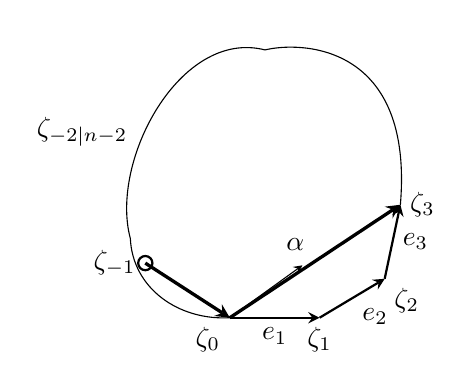
\begin{tikzpicture}[scale=.95,>=stealth]
\coordinate (a) at (-1.65,-.72);
\coordinate (b) at (-.52,-1.45);
\coordinate (c) at (.68,-1.45);
\coordinate (d) at (1.55,-.93);
\coordinate (e) at (1.76,.06);
\draw (e) .. controls (1.94,2.2) and (.45,2.25) .. (-.05,2.13)
 .. controls (-1.18,2.42) and (-2.13,.65) .. (-1.85,-.39)
 .. controls (-1.82,-1.06) and (-1.2,-1.49) .. (b);
\draw[thick] (a) circle (.095);
\draw[->,very thick] (a)--(b);
\draw[->,thick] (b)--node[below]{$e_1$}(c);
\draw[->,thick] (c)--node[below right]{$e_2$}(d);
\draw[->,thick] (d)--node[right]{$e_3$}(e);
\draw[->,very thick] (b)--node[above left]{$\alpha$}(e);
\draw[->] (b)--(.45,-.75);
\node[left] at (-1.76,1.03){$\zeta_{\unsure{-2|n-2}}$};
\node[left] at (a){$\zeta_{-1}$};
\node[below left] at (b){$\zeta_0$};
\node[below] at (c){$\zeta_1$};
\node[below right] at (d){$\zeta_2$};
\node[right] at (e){$\zeta_3$};
\end{tikzpicture}}
